\documentclass[11pt,a4paper]{article}
\usepackage[utf8]{inputenc}
\usepackage[T1]{fontenc}
\usepackage{lmodern}
\usepackage[margin=2cm]{geometry}
\usepackage{amsmath,amssymb}
\usepackage{parskip}
\usepackage{graphicx}
\usepackage[section]{placeins}
\usepackage{hyperref}
\usepackage{listings}
\usepackage{xcolor}
\lstset{language=Python, basicstyle=\ttfamily\scriptsize, columns=fullflexible, keepspaces=true, frame=single, rulecolor=\color{gray!40}, backgroundcolor=\color{gray!5}, showstringspaces=false, upquote=true, xleftmargin=2pt, xrightmargin=2pt}

\newcommand{\T}{^{\mathsf{T}}}
\newcommand{\rot}{{}^{A}_{B}R}

\title{Computer Vision I \\ \large Assignment 1}
\author{Guilherme Guerra Martins \and Maira Alejandra Carvajal Chaparro}
\date{Máster en Intelixencia Artificial · Universidade da Coruña · November 2026}

\begin{document}
\maketitle

% =====================================================================
\section*{Exercise 1}
\emph{Show that the change of coordinates associated with a rigid transformation preserves distances and angles.}

\textbf{Notation.} A point $P$ has coordinates $p$ in the old frame and $p'$ in the new frame. A rigid change of coordinates is a rotation $R$ followed by a translation $t$:
\[
p' = R\,p + t .
\]
Following Hint 1, we take three arbitrary points $P$, $Q$ and $S$.

\textbf{Step 1 --- The key property of a rotation: $R\T R = I$.} The columns of $R$ are the axes of the new frame written in the old one, so they are unit vectors and mutually perpendicular (orthonormal). Entry $(i, j)$ of $R\T R$ is the dot product of column $i$ and column $j$ of $R$. It equals 1 when $i = j$ (a unit vector with itself) and 0 when $i \neq j$ (two perpendicular vectors). Therefore $R\T R = I$. For example, for a rotation of $90^\circ$ in the plane,
\[
R = \begin{pmatrix} 0 & -1 \\ 1 & 0 \end{pmatrix}, \qquad
R\T = \begin{pmatrix} 0 & 1 \\ -1 & 0 \end{pmatrix}, \qquad
R\T R = \begin{pmatrix} 1 & 0 \\ 0 & 1 \end{pmatrix}.
\]

\textbf{Step 2 --- The translation cancels.} Distances and angles are measured on vectors between points, not on single points. Let $u = q - p$ and $v = s - p$ be the two vectors leaving $P$. In the new frame,
\[
u' = q' - p' = (R\,q + t) - (R\,p + t) = R\,(q - p) = R\,u ,
\]
and in the same way $v' = R\,v$. The same $t$ is added to both points and disappears in the subtraction. For example, with the $90^\circ$ rotation and $t = (5, 5)$, the points $p = (1, 0)$ and $q = (3, 0)$ become $p' = (5, 6)$ and $q' = (5, 8)$: every coordinate changes, but $q' - p' = (0, 2) = R\,(2, 0)$ and the distance is 2 in both frames. Only $R$ can still affect lengths and angles.

\textbf{Step 3 --- What must be shown.} Lengths and angles are both computed from dot products:
\[
|u| = \sqrt{u\T u}, \qquad \cos\theta = \frac{u\T v}{|u|\,|v|} .
\]
So we need to check that $R$ changes neither the length of a vector nor the dot product of two vectors.

\textbf{Step 4 --- Distances (Hint 2).} Using $(Ru)\T = u\T R\T$ and Step 1, the length of a vector does not change:
\[
|u'|^2 = (R\,u)\T (R\,u) = u\T (R\T R)\, u = u\T u = |u|^2 .
\]
This is Hint 2, $|AB|^2 = \operatorname{tr}(B\T A\T A B)$, with $A = R$ and $B = u$ (the trace of a $1\times1$ matrix is its only entry). Since lengths are non-negative, $|PQ|' = |PQ|$, and likewise $|PS|' = |PS|$.

\textbf{Step 5 --- Dot products.} The same computation with two different vectors:
\[
u'^{\mathsf{T}} v' = (R\,u)\T (R\,v) = u\T (R\T R)\, v = u\T v .
\]

\textbf{Step 6 --- Angles.} The angle $\theta$ between $PQ$ and $PS$ satisfies
\[
\cos\theta' = \frac{u'^{\mathsf{T}} v'}{|u'|\,|v'|} = \frac{u\T v}{|u|\,|v|} = \cos\theta ,
\]
and since $\theta$ lies in $[0, \pi]$, $\theta' = \theta$.

\textbf{Conclusion.} $P$, $Q$ and $S$ were arbitrary, so the change of coordinates associated with a rigid transformation preserves every distance and every angle.

% =====================================================================
\section*{Exercise 2}
\emph{Derive the formulas for the matrices $\rot$ when $(B)$ is deduced from $(A)$ via a rotation of angle $\theta$ about the axes $\mathbf{i}_A$ ($x$-axis) and $\mathbf{j}_A$ ($y$-axis) respectively.}

\textbf{Idea.} The columns of $\rot$ are the axes of frame $B$ written in frame $A$ (multiplying the matrix by $(1, 0, 0)$ returns its first column, and so on). So the matrix is built by finding where each axis of $A$ lands after the rotation and placing the results as columns. We write $x, y, z$ for $\mathbf{i}_A, \mathbf{j}_A, \mathbf{k}_A$ and $x', y', z'$ for $\mathbf{i}_B, \mathbf{j}_B, \mathbf{k}_B$. A positive angle turns counter-clockwise when the rotation axis points towards the viewer.

\textbf{Method.} For each rotation axis: (1) rotate by $90^\circ$ and find where $x$, $y$ and $z$ land, (2) place $x', y', z'$ as the columns of a $3\times3$ matrix, (3) find the 2D rotation inside that matrix, (4) write it for a general angle $\theta$.

\textbf{Starting case: rotation about $\mathbf{k}_A$ ($z$-axis).}
\[
x = (1,0,0) \to x' = (0,1,0), \qquad
y = (0,1,0) \to y' = (-1,0,0), \qquad
z = (0,0,1) \to z' = (0,0,1).
\]
As columns: $\bigl(\begin{smallmatrix} 0 & -1 & 0 \\ 1 & 0 & 0 \\ 0 & 0 & 1 \end{smallmatrix}\bigr)$.
The top-left $2\times2$ block is the 2D rotation $R(90^\circ) = \bigl(\begin{smallmatrix} 0 & -1 \\ 1 & 0 \end{smallmatrix}\bigr)$, and the fixed axis $z$ adds a 1 with zeros around it. Writing the block for a general angle, $R(\theta) = \bigl(\begin{smallmatrix} \cos\theta & -\sin\theta \\ \sin\theta & \cos\theta \end{smallmatrix}\bigr)$:
\[
R_z(\theta) = \begin{pmatrix} \cos\theta & -\sin\theta & 0 \\ \sin\theta & \cos\theta & 0 \\ 0 & 0 & 1 \end{pmatrix}.
\]

\textbf{Rotation about $\mathbf{i}_A$ ($x$-axis).} Now $x$ is the fixed axis and $y$ turns towards $z$.
\[
x = (1,0,0) \to x' = (1,0,0), \qquad
y = (0,1,0) \to y' = (0,0,1), \qquad
z = (0,0,1) \to z' = (0,-1,0).
\]
As columns: $\bigl(\begin{smallmatrix} 1 & 0 & 0 \\ 0 & 0 & -1 \\ 0 & 1 & 0 \end{smallmatrix}\bigr)$.
The 2D rotation $R(90^\circ)$ is now the bottom-right block, and the fixed axis $x$ gives the 1 in the top-left corner. Writing the block for a general angle:
\[
\rot = R_x(\theta) = \begin{pmatrix} 1 & 0 & 0 \\ 0 & \cos\theta & -\sin\theta \\ 0 & \sin\theta & \cos\theta \end{pmatrix}.
\]

\textbf{Rotation about $\mathbf{j}_A$ ($y$-axis).} Now $y$ is the fixed axis and $z$ turns towards $x$.
\[
x = (1,0,0) \to x' = (0,0,-1), \qquad
y = (0,1,0) \to y' = (0,1,0), \qquad
z = (0,0,1) \to z' = (1,0,0).
\]
As columns: $\bigl(\begin{smallmatrix} 0 & 0 & 1 \\ 0 & 1 & 0 \\ -1 & 0 & 0 \end{smallmatrix}\bigr)$.
The fixed axis $y$ gives the 1 in the centre, and the 2D rotation is spread over the four corners. For a general angle the two turning axes are $x' = (\cos\theta, 0, -\sin\theta)$ and $z' = (\sin\theta, 0, \cos\theta)$, which give the vectors above at $\theta = 90^\circ$:
\[
\rot = R_y(\theta) = \begin{pmatrix} \cos\theta & 0 & \sin\theta \\ 0 & 1 & 0 \\ -\sin\theta & 0 & \cos\theta \end{pmatrix}.
\]

\textbf{Conclusion.} When frame $B$ is obtained from frame $A$ by a rotation of angle $\theta$ about $\mathbf{i}_A$, $\rot = R_x(\theta)$, and about $\mathbf{j}_A$, $\rot = R_y(\theta)$, as derived above. The three cases follow the same pattern: the fixed axis keeps a 1 on the diagonal with zeros in its row and column, and the two axes that turn form a 2D rotation by $\theta$.

% =====================================================================
\section*{Exercise 3}
\emph{Take a picture of a cluttered scenario with the presence of several objects, resize the picture as to be $448\times336$ pixels. Read and show the picture using OpenCV.}

We photographed a cluttered living-room scene (a table with a plant, a laptop, headphones and a notebook, chairs, a sofa, a lamp and a TV) at $5712\times4284$ pixels. The photo is landscape and 4:3, the same proportions as $448\times336$, so both scale factors are equal ($448/5712 = 336/4284 \approx 0.078$) and the objects are not distorted.

Main lines of code. The functions in \texttt{a1\_image.py}:
\begin{lstlisting}
image = cv2.imread(str(path), cv2.IMREAD_COLOR)
if image is None:
    raise FileNotFoundError(f"Could not read image from {path}")

resized = cv2.resize(img, size, interpolation=cv2.INTER_AREA)

cv2.imshow(window, img)
key = cv2.waitKey(0)
cv2.destroyWindow(window)
\end{lstlisting}
and their use on the photo:
\begin{lstlisting}
scene = im.load_bgr(PHOTO)
scene_resized = im.resize_to(scene, (448, 336))
cv2.imwrite(str(DATA_DIR / "scene_448x336.png"), scene_resized)
\end{lstlisting}

\texttt{cv2.imread} returns the image as a (height, width, 3) array in BGR order, and returns \texttt{None} instead of raising an error when it cannot read the file, so \texttt{load\_bgr} raises the error itself. The image goes from shape (4284, 5712, 3) to (336, 448, 3). The size given to \texttt{cv2.resize} is (width, height), the opposite order of the array's shape. \texttt{cv2.imshow} displays the BGR image directly, and \texttt{cv2.waitKey(0)} keeps the window open until a key is pressed.

To shrink, we used \texttt{INTER\_AREA}. Each new pixel stands for about $13\times13$ original pixels. \texttt{INTER\_NEAREST} keeps only one of them, which turns fine detail (the chair fabric, the keyboard) into false patterns (aliasing), while \texttt{INTER\_AREA} averages the whole block. The resized scene is saved as PNG because JPEG would add compression artefacts around edges and texture, which Exercises 4--6 measure.

\begin{figure}[h]
\centering
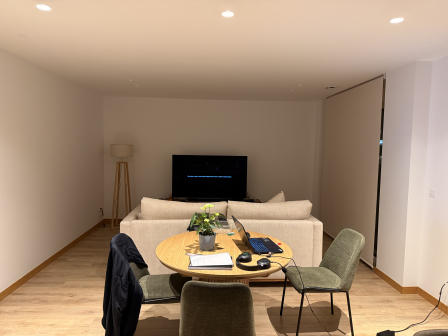
\includegraphics[width=0.31\textwidth]{figures/fig3_scene.png}\hspace{0.02\textwidth}%
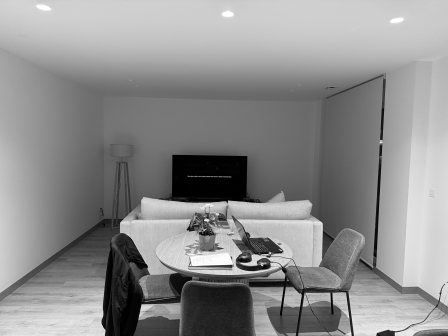
\includegraphics[width=0.31\textwidth]{figures/fig3_gray.png}
\caption{The resized scene, $448\times336$, in colour (left) and grey (right).}
\end{figure}

\section*{Exercise 4}
\emph{Apply a Gabor filter at 4 orientations. Combine (use the maximum value for each pixel) the four orientations into one filtered image and show the result. Play with the parameters of the filter and show how the filter works with 3 different parameter set values.}

A Gabor kernel is a cosine wave inside a Gaussian window: it responds strongly where the image looks like its stripes, with the same width and orientation. We filtered the grey version of the scene (values divided by 255, so all results are on a 0--1 scale) in floating point, because the responses are signed.

Main lines of code (module \texttt{a1\_gabor.py} and its use):
\begin{lstlisting}
def gabor_kernel(ksize, sigma, theta, lambd, gamma, psi=0.0):
    return cv2.getGaborKernel((ksize, ksize), sigma, theta, lambd, gamma, psi, ktype=cv2.CV_32F)

def gabor_bank(gray, params, thetas):
    for theta in thetas:
        kernel = gabor_kernel(**params, theta=theta)
        resp = cv2.filter2D(gray, cv2.CV_32F, kernel)
        responses.append(resp)

def combine_max(responses):
    resp = np.stack(responses, axis=0)
    return resp.max(axis=0).astype(np.float32)

THETAS = np.deg2rad([0, 45, 90, 135])
GABOR_MAX_1_abs = gab.combine_max(abs(gab.gabor_bank(GRAY, SET_1, THETAS)))
\end{lstlisting}

\textbf{Orientations.} $\theta$ is the direction across the stripes, so $\theta = 0^\circ$ has vertical stripes and responds to vertical structures (the lamp legs, the chair legs, the corner of the room), and $\theta = 90^\circ$ responds to horizontal ones (the top of the sofa, the edges of the TV and the table). Turning a kernel by $180^\circ$ gives the same kernel, so the four orientations $0^\circ$, $45^\circ$, $90^\circ$ and $135^\circ$ cover all directions.

\textbf{Combination.} A dark structure on a light background, such as the lamp legs, gives a large \emph{negative} response. With the maximum of the signed responses it disappears, and the background, whose response is about 0, is mapped to a mid grey, so the combined image looks lighter and washed out. We therefore combine the four orientations with the maximum of the absolute values: every oriented structure, bright or dark, stands out on a black background.

\textbf{Three parameter sets.} We changed only the scale, the wavelength $\lambda$ and the window width $\sigma$ (with ksize $\approx 6\sigma$), keeping $\gamma = 0.5$ and $\psi = 0$:
\begin{itemize}\setlength\itemsep{0pt}
\item \textbf{fine} ($\lambda = 4$, $\sigma = 2$): thin, precise outlines, such as the lamp legs, the chair legs, the TV frame and the edges of the table.
\item \textbf{medium} ($\lambda = 8$, $\sigma = 4$): the same objects with thicker, doubled lines, and the thinnest detail is lost.
\item \textbf{coarse} ($\lambda = 16$, $\sigma = 8$): only the large shapes (the sofa, the table, the TV), drawn as wide bands of parallel lines, and the thin legs disappear.
\end{itemize}
The larger the wavelength, the wider the structures the filter responds to.

\begin{figure}[h]
\centering
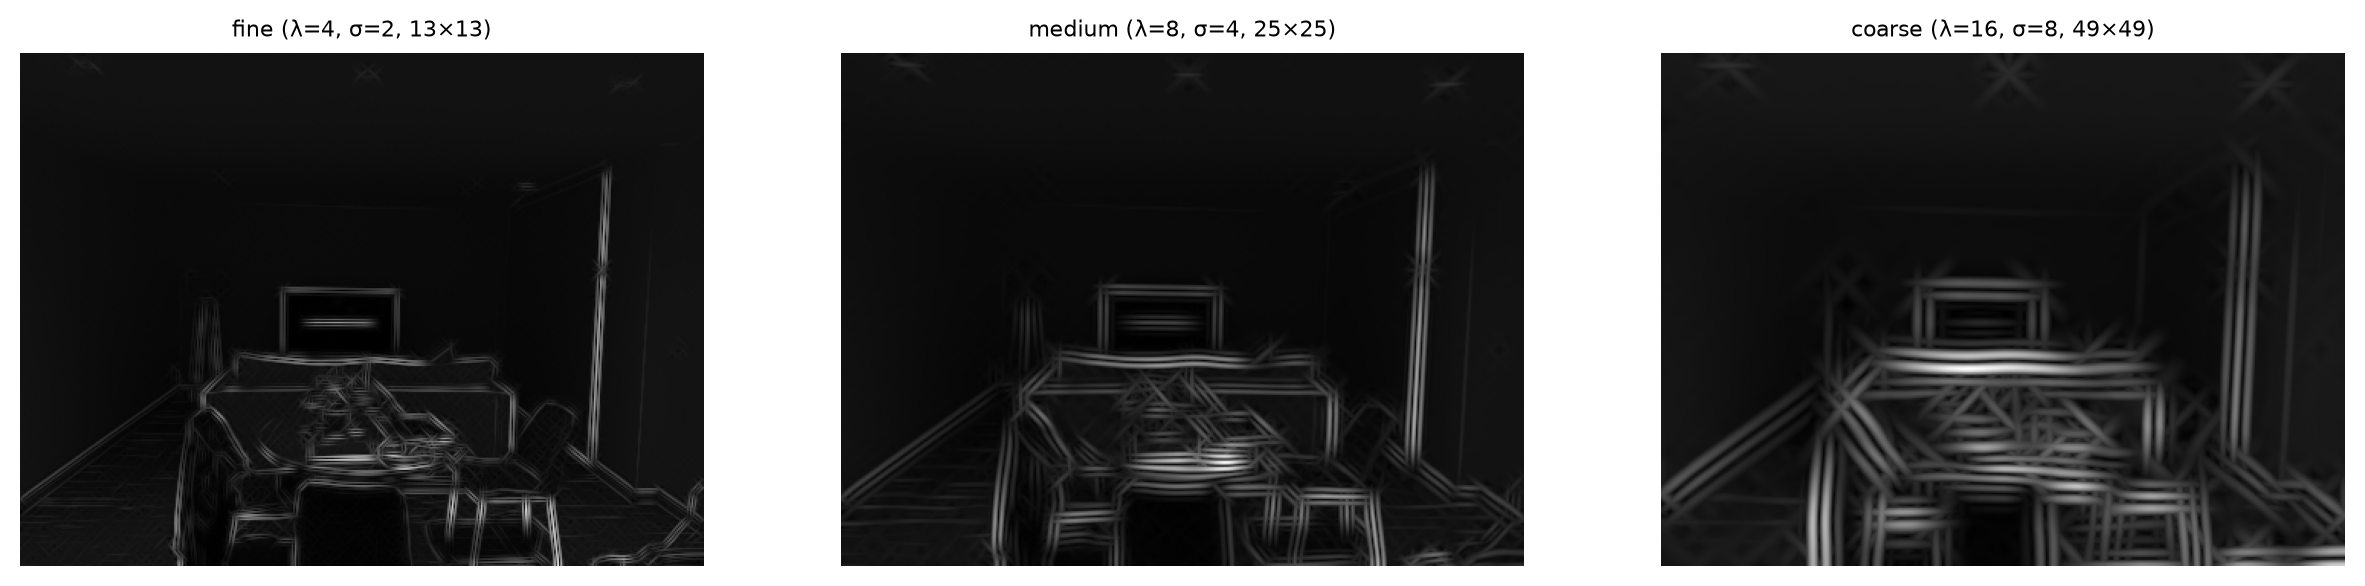
\includegraphics[width=0.82\textwidth]{figures/fig4c_sets.png}
\caption{Gabor filter at 4 orientations, combined by the maximum of the absolute responses, for the three parameter sets.}
\end{figure}

\section*{Exercise 5}
\emph{Apply the Canny Edge detector. Show the result and compare to the result from the Gabor.}

We applied Canny to the grey scene after a Gaussian blur ($5\times5$, $\sigma = 1.4$), with the L2 gradient magnitude:
\begin{lstlisting}
if blur_ksize > 0:
    gray = cv2.GaussianBlur(gray, (blur_ksize, blur_ksize), blur_sigma)
return cv2.Canny(gray, low, high, L2gradient=l2)
CANNY = can.canny_edges(GRAY, 10, 120, blur_ksize=5, blur_sigma=1.4)
\end{lstlisting}

We started from the median heuristic, which gave (low, high) = (99, 196). With this pair the door frame on the right was broken and the floor--wall line was short (Fig.~3). Lowering low to 10 completed these contours, because hysteresis keeps weak pixels that are connected to strong ones. Lowering high to 120 also closed the round table and the chairs, while the walls and the floor stayed empty, so we kept (10, 120). Without the blur, the same pair turned the floor planks, the ceiling lights and the chair fabric into edges: the blur is what keeps texture and noise out.

\begin{figure}[h]
\centering
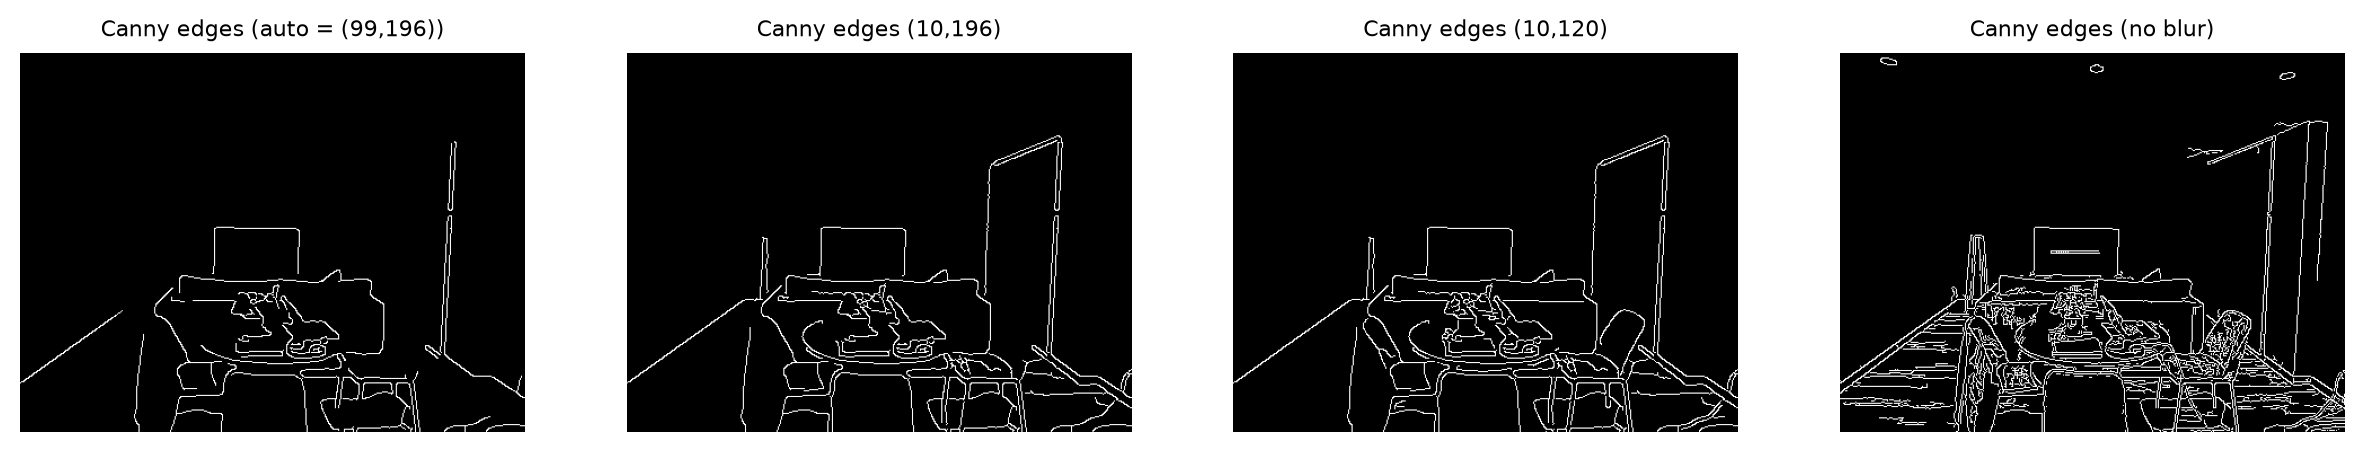
\includegraphics[width=0.9\textwidth]{figures/fig5a_canny.png}
\caption{Canny on our scene: auto (99, 196) $|$ (10, 196) $|$ (10, 120) $|$ (10, 120) without blur.}
\end{figure}

Fig.~4 compares this result with the Gabor bank (fine set, maximum of the absolute responses). Canny gives a binary map of 1-pixel lines, while Gabor gives a continuous response in bands several pixels wide. Both mark dark-on-light and light-on-dark edges, Canny because it uses the gradient magnitude and Gabor because we took the absolute value. They disagree most in two places. On the door frame, Gabor shows a wide band and Canny a single thin line in its middle, because non-maximum suppression keeps only the peak across the edge. On the floor, Gabor responds to the wooden texture while Canny marks nothing, because a Gabor filter is a template of repeated stripes, while Canny looks for individual borders and the blur removes the small ones. Canny is better for locating object outlines, and Gabor for describing oriented patterns and textures.

\begin{figure}[h]
\centering
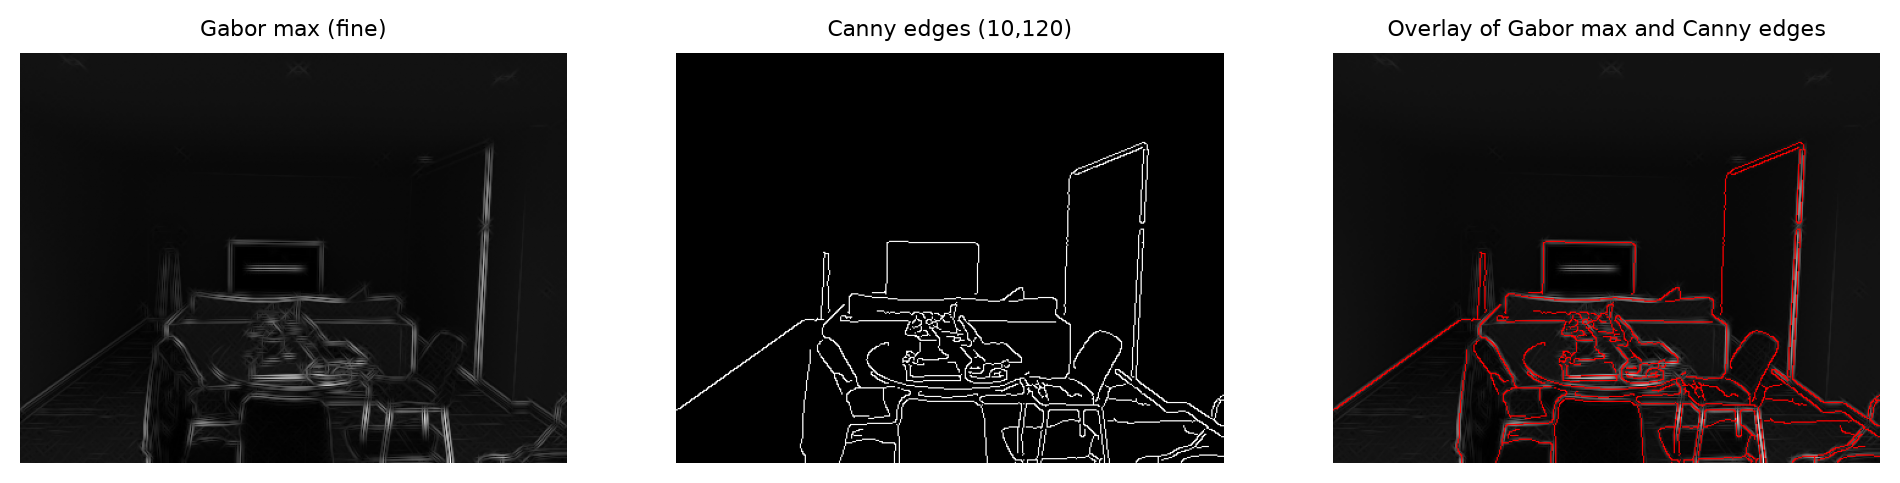
\includegraphics[width=0.78\textwidth]{figures/fig5b_compare.png}
\caption{Gabor maximum (fine set) $|$ Canny (10, 120) $|$ Canny in red over Gabor.}
\end{figure}

\section*{Exercise 6}
\emph{Implement a Gaussian and a Laplacian pyramid. Show the results. Comment on the high and low frequencies and their locations in the results.}

We built both pyramids level by level with OpenCV's REDUCE (\texttt{pyrDown}: blur with $[1,4,6,4,1]/16$, then keep every other pixel) and EXPAND (\texttt{pyrUp}: back to the size of the level below), in float32 because the Laplacian levels are signed. Main lines of \texttt{a1\_pyramids.py}:
\begin{lstlisting}
gauss = [img.astype(np.float32)]
for _ in range(levels):
    gauss.append(cv2.pyrDown(gauss[-1]))
for i in range(len(gauss) - 1):
    h, w = gauss[i].shape[:2]
    expanded = cv2.pyrUp(gauss[i + 1], dstsize=(w, h))
    lap.append(gauss[i] - expanded)
lap.append(gauss[-1].copy())
\end{lstlisting}

Each Gaussian level is the previous one blurred and halved, so it keeps only the lower frequencies (Fig.~5, left). The floor planks and the chair fabric disappear first, then the objects on the table, and $G_4$ ($21\times28$) only shows the layout of the light ceiling and walls against the darker TV and chairs.

Each Laplacian level, $L_i = G_i - \mathrm{EXPAND}(G_{i+1})$, keeps the details that one more blur removes (Fig.~5, right). The high frequencies are in $L_0$, at the floor planks, the chair fabric, the cables, the light bar of the TV and the ceiling lights. The low frequencies are in the top level, $L_4 = G_4$: the smooth walls and ceiling, which are close to zero in every other level.

\begin{figure}[h]
\centering
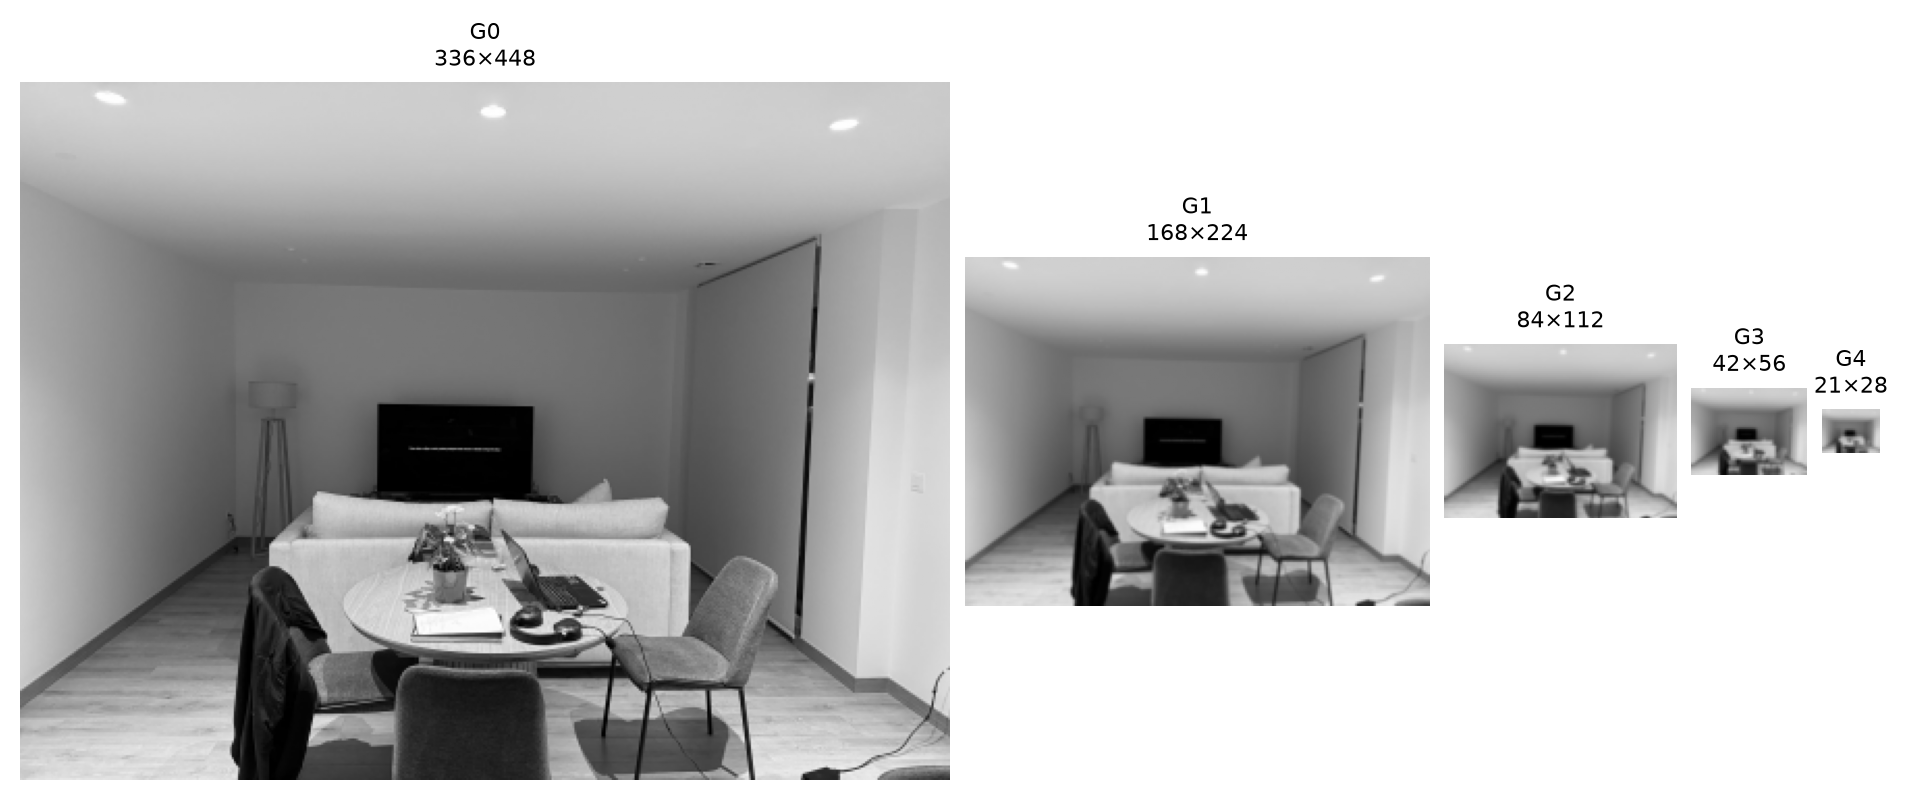
\includegraphics[width=0.495\textwidth]{figures/fig6a_gaussian.png}\hfill
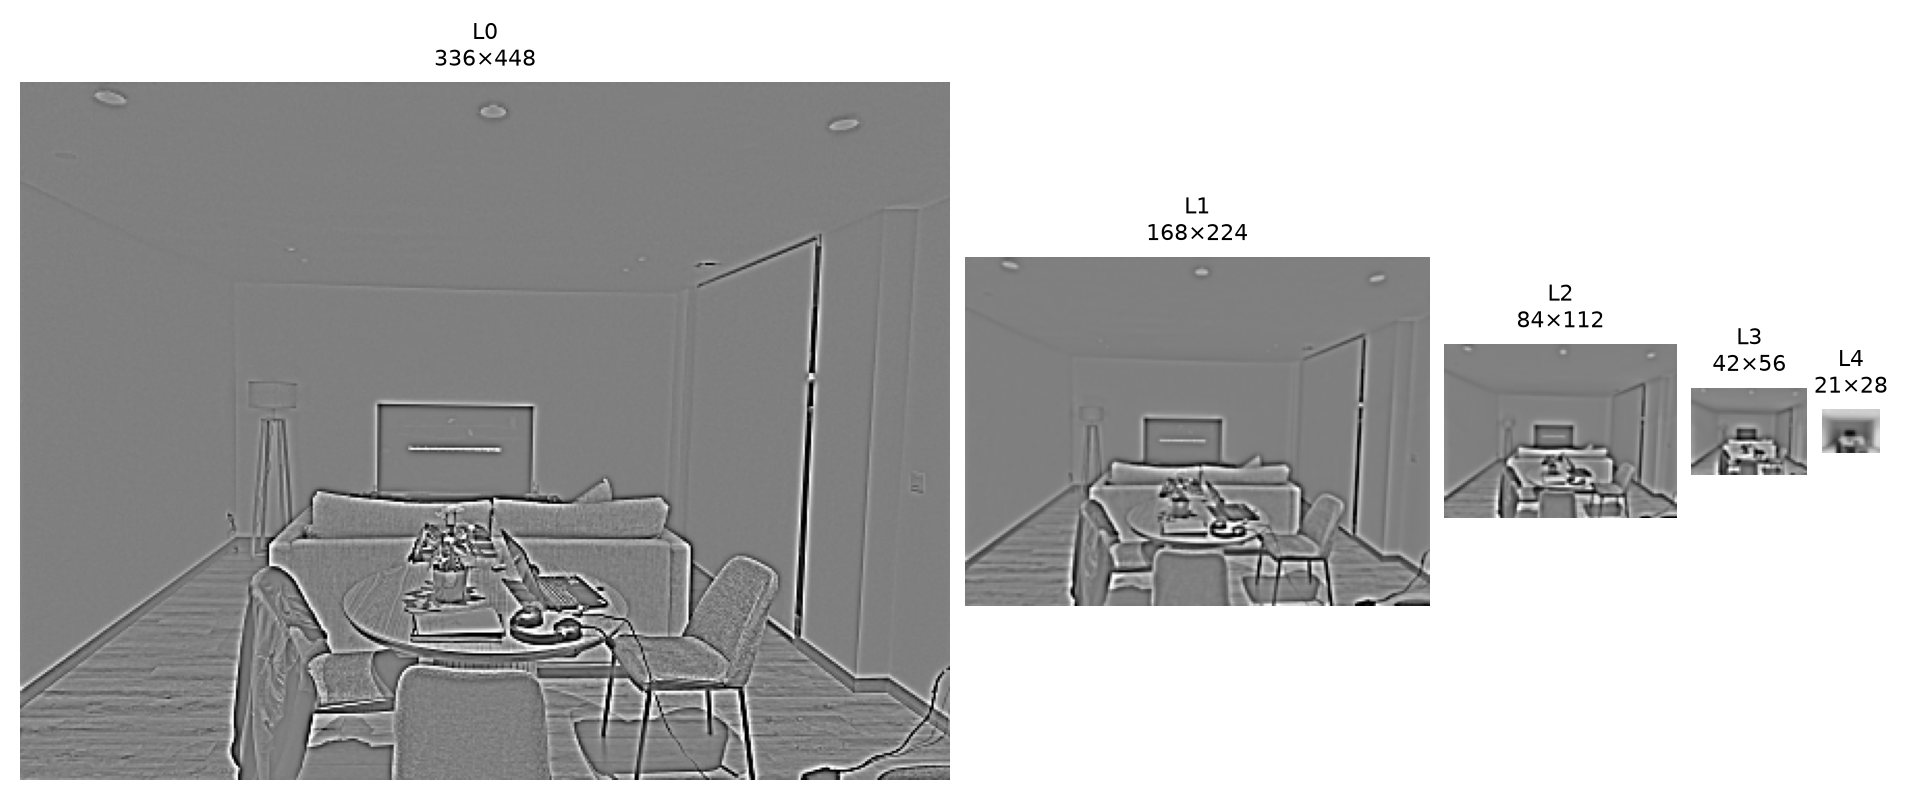
\includegraphics[width=0.495\textwidth]{figures/fig6b_laplacian.png}
\caption{Left: Gaussian pyramid of our scene, from $G_0$ ($336\times448$) to $G_4$ ($21\times28$). Right: Laplacian pyramid, $L_0$--$L_3$ with one shared grey scale (mid-grey $=0$, lighter $=$ positive, darker $=$ negative) and $L_4 = G_4$.}
\end{figure}

\section*{Use of generative AI}
We used Claude (Anthropic) as a study and writing assistant. It explained the theory behind each exercise and the OpenCV and NumPy tools, and helped us structure this report.

\end{document}
